%
% main.tex -- Paper zum Thema <maxwell>
%
% (c) 2020 Autor, OST Ostschweizer Fachhochschule
%
% !TEX root = ../../buch.tex
% !TEX encoding = UTF-8
%

\chapter{Maxwell-Gleichungen als Variationsprinzip\label{chapter:maxwell}}
\kopflinks{Maxwell-Gleichungen als Variationsprinzip}
\begin{refsection}
\chapterauthor{Maurin Doswald und Stephan Oseghale}
\index{Marin Doswald}%
\index{Doswald, Maurin}%
\index{Stephan Oseghale}%
\index{Osghale, Stephan}%

Als James Clerk Maxwell 1865 seine Arbeit über das elektromagnetische Feld veröffentlichte, gelang es ihm, das Wesen des elektrischen- und magnetischen Feldes, sowie die Interaktion derselben mathematisch zu beschreiben und somit das Grundwesen der Elektrodynamik aufzuzeigen.
\index{Maxwell, James Clerk}%
\index{elektrisches Feld}%
\index{magnetisches Feld}%
Durch seine theoretische Arbeit konnte experimentell die Existenz von elektromagnetischen Wellen und ihre Ausbreitung mit Lichtgeschwindigkeit nachgewiesen werden.
\index{Elektrodynamik}%
Dies führte zu Technologien wie Radio, Radar, Fernsehen, Antennen (Kapitel \ref{chapter:antennen}) und viele weitere Anwendungen in der drahtlosen Kommunikation. 
\index{Radio}%
\index{Radar}%
\index{Fernsehen}%
\index{Antennen}%
\index{drahtlos}%
\index{Kommunikation}%
%Eine detaillierte Untersuchung einer weiteren Anwendung wird im Kapitel \ref{chapter:antennen} über Antennen behandelt.

Die Grundidee zur Formulierung dieser Gleichungen kam durch eine Reihe von experimentellen Beobachtungen und theoretischen Ansätzen unterschiedlichster Wissenschaftler unter anderem Michael Faraday und André-Marie Ampère.
\index{Faraday, Michael}%
\index{Ampere, Andre-Marie@Ampère, André-Marie}%
Durch mathematische Analysen und Experimente entwickelte Maxwell schlussendlich zwanzig Gleichungen, welche später von Oliver Heavyside und Willard Gibbs in die heutige bekannte vektorielle Schreibweise von vier Gleichungen gebracht wurden.
\index{Heaviside, Oliver}%
\index{Gibbs, Willard}%
Das Ziel dieser Arbeit ist aufzuzeigen, dass die vier fundamentalen Gleichungen  auch über ein Variationsprinzip hergeleitet werden können.

%
% mathFormulierung.tex -- Felder und deren Operationen
%
% 
%
% !TEX root = ../../buch.tex
% !TEX encoding = UTF-8
%
\section{Felder\label{maxwell:mathFormulierung}}
\rhead{Felder}

Da sowohl das elektrische Feld $\vec{E}$ wie auch das magnetische Feld $\vec{B}$ als Vektorfeld beschrieben werden, soll hier der Begriff des Feldes erläutert und grafisch aufgezeigt werden.

\subsection{Skalarfeld\label{maxwell:skalarfeld}}

Ein Skalarfeld ist eine Funktion der Form
\[ f:\mathbb{R}^n \rightarrow \mathbb{R}, \] 
die jedem Punkt im Raum ein Skalar zuordnet.
Alltägliches Beispiele für ein Skalarfelder sind Temperaturverteilungen, Ladungsdichten oder Potentiale. In \ref{maxwell:skalarGrad} ist der Querschnitt eines Skalarfeldes abgebildet.


%Zu den wichtigsten Operationen eines Skalarfeldes gehört der Gradient, welcher dem Skalar- ein Vektorfeld zuordnet.
%Sei $\phi$ ein Skalarfeld, dann ist $\nabla\phi$ ein Vektorfeld, dargestellt in \ref{maxwell:skalarGrad}.

\begin{figure}
	\centering
	\subfigure{\includegraphics[width=0.35\textwidth]{papers/maxwell/skalar}}
	\subfigure{\includegraphics[width=0.3\textwidth]{papers/maxwell/gradient}}
	\caption{Skalar- und Vektorfeld}
	\label{maxwell:skalarGrad}
\end{figure}

\subsection{Vektorfeld\label{maxwell:vektorfeld}}

Ein Vektorfeld ist eine Funktion der Form \[ f: \mathbb{R}^n \rightarrow \mathbb{R}^m, \] welche jedem Punkt im Raum einen Vektor zuweist. 
Die Richtung dieses Vektors gibt hierbei an, in welche Richtung der Fluss des Feldes an diesem Punkt geht, während der Betrag die Intensität repräsentiert.


Des weiteren spricht man von stationären Vektorfelder, wenn sie zeitunabhängig sind und von homogenen Vektorfelder, wenn die Richtung und der Betrag der Vektoren ortsunabhängig sind, also wenn jeder Vektor die gleiche Richtung und den gleichen Betrag haben. 
Wie bereits erwähnt, sind das elektrische und das magnetische Feld, wie auch andere Kraftfelder Beispiele von Vektorfelder.
Der Querschnitt eines Vektorfeldes ist auch in \ref{maxwell:skalarGrad} abgebildet.

\subsection{Operationen}

\subsubsection{Gradient}

Der Gradient wurde bereits in \ref{buch:fuvar:richtungsableitung:def:gradient} definiert, dieser Operator, welcher auf ein Skalarfeld angewendet wird, resultiert in einem Vektorfeld. 
Die Richtung der Vektoren dieses neuen Vektorfeldes zeigen demnach immer in die Richtung der grössten Zunahme.
%Weiter unten wird ersichtlich, dass auch das elektrische Feld ein Gradientenfeld ist \[ \vec{E} = -\nabla\varphi, \] wobei $\varphi$ das elektrische Potential ist.

\subsubsection{Divergenz}
%TODO: Link auf Kapitel von Müller
Die Divergenz eines Vektorfeldes $\vec{F}$ ist definiert als 
\[ \nabla\cdot\vec{F}. \]
Angewendet wird sie auf ein Vektorfeld und resultiert in ein Skalarfeld.
Die Divergenz sagt aus, ob an einem Punkt mehr ``hinein-'' als ``rausfliesst'' und macht so eine Aussage über das Bestehen von Quellen und Senken.

Wenn die Divergenz negativ ist, liegt eine Senke vor, wenn sie positiv ist eine Quelle.
Ein Vektorfeld wird quellenfrei genannt, wenn seine Divergenz zu null resultiert.

\subsubsection{Rotation}
%TODO: Link auf Kapitel von Müller
Die Rotation eines Vektorfeldes $\vec{F}$ ist definiert als,
\[ \nabla\times\vec{F}. \]
Mit dieser Operation wird einem Vektorfeld ein neues Vektorfeld zugeordnet, welches eine Aussage macht, wie stark das Feld sich um einen Punkt dreht bzw. rotiert.
Wenn die Rotation zu null resultiert, ist das Feld wirbelfrei.

%
% einleitung.tex -- Beispiel-File für die Einleitung
%
% (c) 2020 Prof Dr Andreas Müller, Hochschule Rapperswil
%
% !TEX root = ../../buch.tex
% !TEX encoding = UTF-8
%
% erste Maxwellgleichung ohne Quelle

\tikzset{>=latex} % for LaTeX arrow head
\usetikzlibrary {arrows.meta}
\pgfplotsset{compat=1.13}
\usetikzlibrary{decorations.markings,intersections,calc}
\usetikzlibrary{angles,quotes} % for pic (angle labels)
\colorlet{Ecol}{green!90!black}
\colorlet{EcolFL}{green!80!black}
\colorlet{Bcol}{blue!90!black}
\tikzstyle{EcolEP}=[blue!80!white]
\colorlet{veccol}{green!45!black}
\tikzstyle{charge+}=[very thin,top color=red!50,bottom color=red!90!black,shading angle=20]
\tikzstyle{charge-}=[very thin,top color=blue!50,bottom color=blue!80,shading angle=20]
\tikzstyle{charge_small} = [very thin,top color=red!50,bottom color=red!90,shading angle=20]
\tikzstyle{vector}=[->,thick,veccol]
\tikzset{EFieldLineArrow/.style={EcolFL,decoration={markings,mark=at position #1 with {\arrow{latex}}},
		postaction={decorate}},
	EFieldLineArrow/.default=0.5}


\section{Elektrostatik\label{maxwell:section:elekktrostatik}}
\rhead{Elektrostatik}
Die Elektrostatik ist ein Spezialfall der Elektrodynamik, bei dem statische Felder betrachtet werden.
Dies setzt voraus, dass
\begin{equation}
	\frac{\partial f}{\partial t}
	=
	0
	\qquad
	\forall f,t.
	\label{maxwell:section:definition_statik}
\end{equation}
Daraus folgt, dass wir nur ruhende Ladungen betrachten.
Dies hat zur Folge, dass keine Stromdichten existieren können, weil
\begin{equation}
	\rho(x,y,z) \underbrace{\vec{v}}_{=0}
	=
	\vec{j}(x,y,z)
	=
	0.
\end{equation}
Im späteren Abschnitt \ref{maxwell:magnetostatik} der Magnetostatik wird klar, dass aus diesem Grund in der Elektrostatik keine magnetische Flussdichte existieren kann.
 
Das Ziel ist nun das elektrische Feld im Zusammenspiel mit ruhenden Ladungen zu beschreiben.
Dafür werden wir in den folgenden Abschnitten die nötigen Begriffe definieren und genauer erklären.

%TODO: Ladung noch definieren? (denke nicht)
\subsubsection{Elektrisches Potentialfeld}
Das elektrische Potentialfeld
\[
\phi:\mathbb{R}^3
\rightarrow
\mathbb{R}
\]
ist als
\begin{equation}
	\phi(x,y,z)
	=
	\frac{W_{pot}(x,y,z)}{q}
	\label{maxwell:section:definition_elektrischespotentialfeld}
\end{equation}
definiert.
In Worten gefasst kann man sagen, dass das elektrische Potential eine auf Ladung normierte, potentielle Energie darstellt.
Somit kann die linke Abbildung in \ref{maxwell:skalarGrad} als ein Feld, das proportional zur potentiellen Energie ist, angeschaut werden.
Des Weiteren steht die elektrische Spannung eng in Verbindung mit dem elektrischen Potential.
Die Spannung $U$ zwischen zwei Punkten $a$ und $b$ wird definiert als
\[
U_{ab}
=
\phi_a - \phi_b.
\]
% not sure about this
Das heisst die Spannung ist der Potentialunterschied zwischen zwei Punkten.

\subsubsection{Elektrisches Feld}
Das elektrische Feld
\[
\vec{E}:\mathbb{R}^3 \rightarrow \mathbb{R}^3
\]
wird ganz allgemein definiert als
\begin{equation}
\vec{E}(x,y,z)
=
- \nabla\phi(x,y,z) - \frac{\partial \vec{A}}{\partial t}(x,y,z),
\label{maxwell:section:definiton_allgemein_elektrischesFeld}
\end{equation}
wobei $\vec{A}$ das magnetische Vektorpotential ist \eqref{maxwell:definitionVektorpot}.
Da wir dank Gleichung \eqref{maxwell:section:definition_statik} wissen, dass alle zeitlichen Ableitungen null sein müssen, ist die statische Definition des elektrischen Feldes
\begin{equation}
\vec{E}(x,y,z)
=
- \nabla\phi(x,y,z).
\label{maxwell:section:definition_statisch_elektrischesFeld}
\end{equation}
Diese Definition besagt, dass das elektrische Feld ein statisches Gradientenfeld ist.
Dieses Feld kann man anhand der Kraftwirkung an sogenannten Probeladungen $q$ messen, da
\[
\vec{E}(x,y,z)
=
\frac{\vec{F}(x,y,z)}{q}
\]
ist.
Somit sind die Vektoren in Abbildung \ref{maxwell:section:E-Feld_punktladung} Kraft Vektoren, welche normiert sind auf die Ladung $q$.
%E-Field of point charge
\begin{figure}[h]
	\centering
	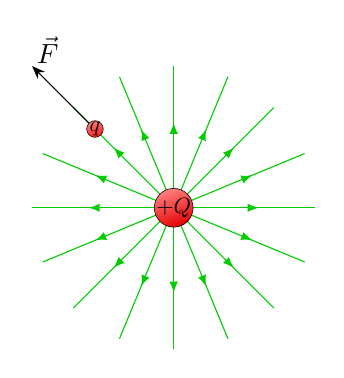
\begin{tikzpicture}
		\def\R{1.8}
		\def\NE{16}
		\def\NV{4}
		\contourlength{1.6pt}
		
		\foreach \i [evaluate={\angle=(\i-1)*360/\NE;}] in {1,...,\NE}{
			\draw[EFieldLineArrow={0.6}] (0,0) -- (\angle:\R);
		}
		\draw[charge+] (0,0) circle (7pt) node[black,scale=0.8] {$+Q$};
		%\draw[FFieldLineArrow={0.6}] (-1,1) -- (-2,2);
		\draw[-{Stealth[black]}] (-1,1) -- (-1.8,1.8) node at (-1.6, 2) {$\vec{F}$};
		\draw[charge_small] (-1,1) circle (3pt) node[black,scale=0.8] {$q$};
	\end{tikzpicture}
	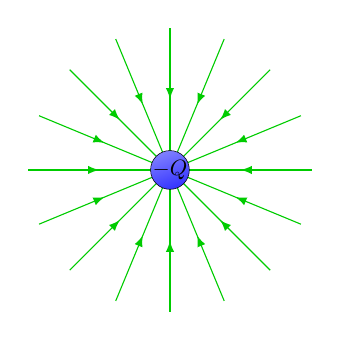
\begin{tikzpicture}
		\def\R{1.8}
		\def\NE{16}
		\def\NV{4}
		\contourlength{1.6pt}
		
		\foreach \i [evaluate={\angle=(\i-1)*360/\NE;}] in {1,...,\NE}{
			\draw[EFieldLineArrow={0.5}] (\angle:\R) -- (0:0);
		}
		\draw[charge-] (0,0) circle (7pt) node[black,scale=0.8] {$-Q$};
	\end{tikzpicture}
	\caption{Elektrisches Feld einer positiven-/ negativen Punktladung}
	\label{maxwell:section:E-Feld_punktladung}
\end{figure}

\subsubsection{Energiedichte im elektrischen Feld}
Das elektrische Feld beinhaltet eine Energie und somit auch eine Energiedichte.
Diese Energiedichte ist definiert als
\begin{equation}
w_e
=
\frac{1}{2} \epsilon \vec{E} ^2,
\label{maxwell:section:definiton_energiedichte_elektrischesFeld}
\end{equation}
wobei $\epsilon$ die Permittivität ist.
Die Permittivität
\[
\epsilon
=
\epsilon_r \epsilon_0
\]
ist das Produkt der relativen Permittivität $\epsilon_r$ und der Permittivität von Vakuum $\epsilon_0$.
Die relative Permittivität ist eine materialabhängige Grösse und hat in Vakuum den skalaren wert $1$.
Die Permittivität von Vakuum
\[
\epsilon_0
=
8.854 \cdot 10^{-12} F/m
\]
ist die elektrische Feldkonstante.


\subsection{Gausssches Gesetz quellenfrei
	\label{maxwell:section:elektrostatik_ohne_quelle}}
\rhead{Problemstellung}
Man stelle sich nun einen ladungsfreien, luftleeren, drei dimensionalen Raum $V\subset\mathbb{R}^3$
vor, indem ein elektrisches Potentialfeld $\phi(x,y,z)$ existiert.
Für diesen Raum möchten wir mittels der Varitaionsrechnung eine Gleichung entwickeln, die beschreibt, wie sich das Potentialfeld verhählt. 

\subsubsection{Ansatz}
Damit wir eine Gleichung erhalten, die das Verhalten des elektrischen Potentialfeldes beschreibt, muss ganz allgemein die Energie im System minimiert werden. 
In diesem Fall ist die Energie im System
\[
W_e
=
\iiint_V w_e\, dV.
\]
Dieses Integral gilt es zu minimieren, was die Grundlage für unser Variationsproblem darstellt.
Die in \eqref{maxwell:section:definiton_energiedichte_elektrischesFeld} definierte Energiedichte ist in Vakuum
% TODO: Bei definitionen erwähnen, dass ein vektor v^2 = v dot v ist!
\[
w_e\
=
\frac{1}{2}\epsilon_0\vec{E}(x,y,z)^2.
\]
Diese Gleichung können wir nun mittels definition \eqref{maxwell:section:definition_statisch_elektrischesFeld} mit dem elektrischen Potentialfeld ausdrücken.
somit ist
\begin{align}
\renewcommand{\arraystretch}{1.9}
w_e
&=
\frac{1}{2}\epsilon_0\left(-\nabla\phi(x,y,z)\right)^2
\\
w_e
&=
\frac{1}{2}\epsilon_0
\begin{pmatrix}
\displaystyle
-\phi_x\\
\displaystyle
-\phi_y\\
\displaystyle
-\phi_z
\end{pmatrix}
\cdot
\begin{pmatrix}
\displaystyle
-\phi_x\\
\displaystyle
-\phi_y\\
\displaystyle
-\phi_z
\end{pmatrix}
\\
w_e
&=
\frac{1}{2}\epsilon_0\left(\phi_x^2 + \phi_y^2 + \phi_z^2\right).
\label{maxwell:section:energiedichte}
\end{align}
Dies können wir in das zu minimerende Integral einsetzen und bekommen
%TODO: eventuell underbraces weg lassen.
\begin{equation}
	W_e
	=
	\iiint_V \underbrace{
		\frac{1}{2}\epsilon_0\left(\phi_x^2 + \phi_y^2 + \phi_z^2\right)}_{L(x,y,z,\phi,\phi_x,\phi_y,\phi_z)}\, dV.
	\label{maxwell:section:energieintegral_quellenfrei}
\end{equation}
Aus dieser Gleichung können wir entnehmen, dass unsere Lagrangefunktion
\begin{equation}
	L(x,y,z,\phi,\phi_x,\phi_y,\phi_z)
	=
	\frac{1}{2}\epsilon_0\left(\phi_x^2 + \phi_y^2 + \phi_z^2\right)
	\label{maxwell:section:lagrangefunktion_quellenfrei}
\end{equation}
ist.
Somit haben wir unsere Lagrangefunktion gefunden, die wir in einem nächsten Schritt in die Euler-Ostrogradski-Differentialgleichung einsetzen können.

\subsubsection{Einsetzen in die Euler-Ostrogradski-Differentialgleichung}
%TODO: label suchen von E-O-DGL von müller kapitel
Nun gilt es die in \eqref{maxwell:section:lagrangefunktion_quellenfrei} gefundene Gleichung in die E-O-DGL \ref{???} einzusetzen.
Nach Einsetzen wird die Differentialgleichung
\[
\frac{1}{2}\epsilon_0\left(\underbrace{\frac{\partial}{\partial\phi}\left(\phi_x^2 + \phi_y^2 + \phi_z^2\right)}_{=0} - \frac{\partial}{\partial x}\frac{\partial}{\partial \phi_x}\left(\phi_x^2 + \phi_y^2 + \phi_z^2\right) - 
\frac{\partial}{\partial y}\frac{\partial}{\partial \phi_y}\left(\phi_x^2 + \phi_y^2 + \phi_z^2\right) - 
\frac{\partial}{\partial z}\frac{\partial}{\partial \phi_z}\left(\phi_x^2 + \phi_y^2 + \phi_z^2\right)\right)
=
0.
\]
Man sieht, dass die partielle Ableitung nach $\phi$ verschwindet.
Nach den partiellen Ableitungen nach $\phi_x$, $\phi_y$ und $\phi_z$ wird die Differentialgleichung
\[
\frac{1}{2}\epsilon_0\left(-\frac{\partial}{\partial x}2\phi_x - \frac{\partial}{\partial y}2\phi_y - \frac{\partial}{\partial z}2\phi_z\right)
=
0.
\]
Wenn man nun noch die letzten partiellen Ableitungen macht, wird die Differentialgleichung
\begin{equation}
	- \underbrace{\epsilon_0}_{\not{=}0}\underbrace{\left(\frac{\partial^2\phi}{\partial x^2} + \frac{\partial^2\phi}{\partial y^2} + \frac{\partial^2\phi}{\partial z^2}\right)}_{=0}
	=
	0.
	\label{maxwell:section:laplace_gleichung_1}
\end{equation}
%definiton des laplace operators suchen
An dieser Gleichung sieht man, dass die Klammer mit den partiellen Ableitungen gleich null sein muss, da die Permittivität von Vakuum nicht null sein kann.
Zusätzlich wird nun ersichtlich, dass der Klammerterm nach definition \ref{???} mit dem Laplace-Operator angewendet auf das elektrische Potentialfeld $\phi$ ersetzt werden kann.
Somit wird unsere schluss Differentialgleichung
\begin{equation}
	\Delta\phi
	=
	0.
	\label{maxwell:section:laplace_gleichung_2}
\end{equation}
Durch Anwendng der Definiton des Laplace-Operator \ref{???} und der Definiton des elektrischen Feldes \eqref{maxwell:section:definition_statisch_elektrischesFeld} erhalten wird die Gleichung
\[
\nabla\cdot\underbrace{\nabla\phi}_{-\vec{E}}
=
0.
\]
Hiermit erhalten wir, dass
\begin{equation}
	\nabla\cdot\vec{E}
	=
	0
	\label{maxwell:section:e_feld_quellenfrei}
\end{equation}
% TODO:Bild referenz einfügen und Bild erstellen
sein muss. Diese Differentialgleichung besagt, dass das elektrische Feld quellenfrei ist.
Dies bedeutet, dass Felldlinien des elektrischen Feldes an keinem Ort im Raum enstehen oder enden können.
Dies ist sehr naheliegend, da ohne Ladungen im Raum das elektrische Feld quellenfrei sein muss.

%Darf auch weggelassen werden.
\subsubsection{Exkurs zur Laplace-Gleichung}
\label{maxwell:section:laplacegleichung_exkurs}
Ein Potentialfeld, das die Laplace-Gleichung
\[
-\Delta\varphi
=
0
\]
erfüllt, führt zu einem Gradientenfeld $\nabla\varphi$, das rotationsfrei und quellenfrei ist.
Diese Gleichung findet nicht nur Anwendungen in der Elektrostatik, sondern auch in stationärer Fluiddynamik und stationärer Wärmeleitung.







%
% einleitung.tex -- Beispiel-File für die Einleitung
%
% (c) 2020 Prof Dr Andreas Müller, Hochschule Rapperswil
%
% !TEX root = ../../buch.tex
% !TEX encoding = UTF-8
%
%erste Maxwell Gleichung mit Quelle
\subsection{Gausssches Gesetz
\label{maxwell:section:elektrostatik_mit_quelle}}
\rhead{Problemstellung}
Nun betrachten wir einen luftleeren, dreidimensionalen Raum $V\subset\mathbb{R}^3$, in dem ein elektrisches Potentialfeld $\phi(x,y,z)$ und eine Ladungsdichte $\varrho(x,y,z)$ existieren.
Auch für diesen Raum möchten wir mittels Variationsrechnung eine Gleichung finden, die das Verhalten des elektrischen Potentialfeldes beschreibt.

\subsubsection{Ansatz}
\rhead{Ansatz}
Es ist naheliegend, dass auch in diesem Szenario die Energie im System minimiert werden muss.
Wie auch in Gleichung \eqref{maxwell:section:energieintegral_quellenfrei} ist die Energie im elektrischen Feld
\[
W_e
=
\iiint_V \frac{1}{2}\,\varepsilon_0\,(\phi_x^2 + \phi_y^2 + \phi_z^2)\, dV.
\]
Jedoch ist dies nicht die einzige Komponente der gesamt Energie des Systems.
Laut \eqref{maxwell:section:definition_elektrischespotentialfeld} ist das elektrische Potential eine auf die Ladung normierte potentielle Energie.
Somit haben wir die fehlende Komponente gefunden.
Damit wir die durch die Ladung
\begin{equation}
q
=
\iiint_V \varrho(x,y,z)\, dV
\label{maxwell:ladung}
\end{equation}
verursachte potentielle Energie $W_q$ im System mit der Ladungsdichte $\varrho$ ausdrücken können, müssen wir untersuchen, was eine infinitesimale potentielle Energie verursacht.
Wenn wir diese infinitesimal kleine potentielle Energie
\(
dW_q
=
\phi\, dq
\)
unter die Lupe nehmen und für die infinitesimal kleine Ladung
\(
dq
=
\varrho\, dV
\)
einsetzen, erhalten wir
\(
dW_q
=
\phi\,\varrho\, dV.
\)
Jetzt müssen die infinitesimalen potentiellen Energien im Raum $V$ zusammengezählt werden und es resultiert
\begin{equation}
W_q
=
\iiint_V \varrho\,\phi\, dV.
\label{maxwell:section:potenzielle_energie_ladung}
\end{equation}
Mit der Gesamtenergie
\[
W_{tot}
=
W_e - W_q
=
\iiint_V \frac{1}{2}\,\varepsilon_0\left(\phi_x^2 + \phi_y^2 + \phi_z^2\right) - \phi\,\varrho\, dV
\]
des Systems haben wir unser zu minimierendes Integral gefunden.
Daraus können wir wieder die Lagrange-Funktion
\begin{equation}
L(x,y,z,\phi,\phi_x,\phi_y,\phi_z)
=
\frac{1}{2}\,\varepsilon_0\left(\phi_x^2 + \phi_y^2 + \phi_z^2\right) - \phi\,\varrho
\label{maxwell:section:lagrangefunktion_mit_quelle}
\end{equation}
% TODO: Müller fragen wegen kopplungsterme
ablesen.
Man bemerkt, dass die Lagrange-Funktion einen zusätzlichen additiven Term erhalten hat im Verlgeich zur Lagrange-Funktion \eqref{maxwell:section:lagrangefunktion_quellenfrei}.
Solche Terme nennt man Kopplungsterme.
Sie werden verwendet, um die Wechselwirkung zwischen Termen in der Lagrange-Funktion zu berücksichtigen.
Der Kopplungsterm in unserem Fall beschreibt die Wechselwirkung zwischen dem Feld und der Ladungsdichte.
Nun können wir diese Lagrangefunktion in die Euler-Ostrogradski-Differentialgleichung einsetzen, um zu untersuchen, wie sich das elektrische Potentialfeld verhält.

\subsubsection{Einsetzen in die Euler-Ostrogradski-Differentialgleichung}
Nun wollen wir die in \eqref{maxwell:section:lagrangefunktion_mit_quelle} gefundene Lagrangefunktion in die Euler-Ostrogradski-Differentialgleichung einsetzten.
Um die Rechnung übersichtlicher zu gestalten, machen wir uns die Linearität der Euler-Ostrogradski-Differentialgleichung
\begin{equation}
F\left\{W_{tot}\right\}
=
F\left\{W_e - W_q\right\}
=
F\left\{W_e\right\} + F\left\{-W_q\right\}
\label{maxwell:section:linearität_von_DGL}
\end{equation}
zu nutze.
Die Lösung von $F\left\{W_e\right\}$ haben wir in Gleichung \eqref{maxwell:section:laplace_gleichung_1} bereits gefunden.
Durch einsetzen von $-W_q$ in die Euler-Ostrogradski-Differentialgleichung erhalten wir
\[
\frac{\partial}{\partial\phi}\left(-\varrho\,\phi\right) - \underbrace{\frac{\partial}{\partial x}\frac{\partial}{\partial\phi_x}\left(\varrho\,\phi\right)}_{=0} - \underbrace{\frac{\partial}{\partial y}\frac{\partial}{\partial\phi_y}\left(\varrho\,\phi\right)}_{=0} - \underbrace{\frac{\partial}{\partial z}\frac{\partial}{\partial\phi_z}\left(\varrho\,\phi\right)}_{=0}
=
0.
\]
Da alle partiellen Ableitungen nach $\phi_x, \phi_y, \phi_z$ null ergeben, müssen wir nur noch die partielle Ableitung nach $\phi$ erledigen.
Somit ist
\(
-\varrho
=
0.
\)
Durch Addition unserer zwei Teillösungen erhalten wir die Gleichung
\begin{align*}
-\varepsilon_0\,\Delta\phi - \varrho
&=
0
\\
\Leftrightarrow \qquad \varepsilon_0\,\Delta\phi
&=
-\varrho.
\end{align*}
Schlussendlich erhalten wir
\begin{equation}
\Delta\phi
=
-\frac{\varrho}{\varepsilon_0}.
\label{maxwell:section:erste_maxwellgleichung_1}
\end{equation}
% TODO: definiton des laplace-operators suchen
Durch gleiches Vorgehen wie in Gleichung \eqref{maxwell:section:laplace_gleichung_3} erhalten wir
\[
\nabla\cdot\underbrace{\nabla\phi}_{\displaystyle-\vec{E}}
=
-\frac{\varrho}{\varepsilon_0}.
\]
Somit können wir erneut die Schlussdifferentialgleichung mit dem elektrischen Feld ausdrücken. Dadurch muss
\begin{equation}
\nabla\cdot\vec{E}
=
\frac{\varrho}{\varepsilon_0}
\label{maxwell:section:erste_maxwellgleichung_2}
\end{equation}
gelten.
Wir sehen, dass dies der ersten Maxwell-Gleichung in differentieller Schreibweise entspricht.

\subsubsection{Interpretation des Resultates}
Die erste Maxwell-Gleichung \eqref{maxwell:section:erste_maxwellgleichung_2} besagt, dass die Quelle des elektrischen Feldes eine Ladungsdichte $\varrho$ ist.
Dies bedeutet, dass elektrische Feldlinien auf Ladungen enden können.
In anderen Worten wird das elektrostatische Feld durch Ladungen erzeugt!
Da es sowohl positive wie auch negative Ladungen gibt, gilt dasselbe für die Ladungsdichten.
Wenn die Ladungsdichte positiv ist, sagt uns die erste Maxwell-Gleichung, dass das elektrische Feld eine Quelle besitzt.
Das heisst, salopp gesagt, die Feldvektoren zeigen weg von der Ladungsdichte.
Wenn die Ladungsdichte jedoch negativ ist, besitzt das elektrische Feld eine Senke.
Das heisst in diesem Fall, dass die Feldvektoren auf die Ladungsdichte zeigen. Dies ist in Abbildung \ref{maxwell:section:E-Feld_punktladung} veranschaulicht.

\subsubsection{Exkurs zur Poisson-Gleichung}
% Darf auch weggelassen werden.
Die Poisson-Gleichung
\[
\Delta\phi
=
f,
\]
wobei $\phi$ ein Potentialfeld und $f$ eine Quelle ist, findet in vielen Teilen der Physik ihre Anwendungen.
Die Quelle $f$ kann wie in Gleichung \eqref{maxwell:section:erste_maxwellgleichung_1} eine Funktion des Raumes und/oder eine Funkiton der Zeit sein.
Ein Potentialfeld, dass die Poisson-Gleichung erfüllt, führt zu einem Gradientenfeld $\nabla\varphi$, dass die Quelle $f$ besitzt und Rotationsfrei ist.
Die homogene Gleichung, also wo $f = 0$ ist, führt uns zur Laplace-Gleichung.








%
% magnetostatik.tex -- Herleitung Amperesches Gesetz über E-O-DGL
%
% (c) 2020 Prof Dr Andreas Müller, Hochschule Rapperswil
%
% !TEX root = ../../buch.tex
% !TEX encoding = UTF-8
%
\section{Magnetostatik\label{maxwell:magnetostatik}}
\rhead{Magnetostatik}



In der Magnetostatik betrachten wir stationäre magnetische Felder.
Die Ursache eines stationären magnetischen Feldes sind Permanentmagnete oder Gleichströme also bewegte Ladungen.
Wir setzen also neu
\[ 
\frac{\partial q}{\partial t}
=
I
=
\text{const}
\qquad
\forall
q,t
\]
voraus.
Zusätzlich konzentrieren wir uns in diesem Abschnitt ausschliesslich auf das magnetische Feld bzw. die magnetische Flussdichte, somit wird auch 
\[\phi(x,y,z) = 0 \qquad \forall x,y,z\] 
angenommen.

Fliesst ein konstanter Strom in einem Leiter, so erzeugt dieser ein Magnetfeld konzentrisch um den geraden Leiter, wie in Abbildung \ref{maxwell:flussdichte} abgebildet ist.
Aufgrund des nicht existieren magnetischer Monopole schliessen sich die Feldlinien des magnetischen Feldes vollständig, was bedeutet, dass das Feld keine Quellen aufweist und somit quellenfrei ist.

\begin{figure}
\centering
% WIRE B FIELD 3D
\begin{tikzpicture}[z={(0.8,0.28)},x={(0.58,-0.45)}]
	
	\def\L{6}
	\def\W{0.10}
	\def\R{0.9}
	\def\ang{-35}
	\def\scale{1.3}
	\def\NB{5}
	\coordinate (O) at (0,0,0);
	%\draw (0,0,0) -- (2,0,0);
	%\draw (0,0,0) -- (0,0,2);
	
	% Koordinatensystem
	\draw[->] (0,0,0) -- (3,0,0) node[anchor=north east]{$x$};
	\draw[->] (0,0,0) -- (0,3,0) node[anchor=north west]{$z$};
	\draw[->] (0,0,0) -- (0,0,4) node[anchor=south]{$y$};
	
	% B FIELD BACK
	\foreach \i [evaluate={\x=(\i-\NB/2-0.5)*\L/\NB;}] in {1,...,\NB}{
		%\draw[BField,-] (0,0,\x)++(\ang+1:\R) arc (\ang+1:\ang-181:\R);
		\draw[BFieldLine=1] (0,0,\x)++(\ang+1:\R) arc (\ang+1:\ang-181:\R) --++ (65:0.001*\R);
	}
	
	% WIRE
	\draw[metal] (0,0,-\L/2)++(120:\W/2) --++ (0,0,\L) arc (120:-60:\W/2) --++ (0,0,-\L) arc (-60:120:\W/2);
	\draw[metal] (0,0,-\L/2) circle (\W/2);
	\draw[current] (0.12*\R,-0.12*\R,0.4*\L) --++ (0,0,0.2*\L) node[below=2,right] {$I$};
	
	% B FIELD FRONT
	\foreach \i [evaluate={\x=(\i-\NB/2-0.5)*\L/\NB;}] in {1,...,\NB}{
		%\draw[BFieldLine=1] (0,0,\x)++(\ang+180:\R) arc (\ang+180:\ang:\R) --++ (-116:0.001*\R);
		\draw[BField,-] (0,0,\x)++(\ang+180:\R) arc (\ang+180:\ang:\R);
	}
	\node[Bcol] at (-0.9*\R,0.9*\R,-0.25*\L) {$\vec{B}$}; %++(140:1.3*\R)
	
\end{tikzpicture}
	\caption{Magnetische Flussdichte um einen geraden Leiter}
	\label{maxwell:flussdichte}
\end{figure}




\subsubsection{Magnetisches Vektorpotential}

Das magnetische Vektorpotential ist ein Vektorfeld, mit welchem die magnetische Flussdichte als 
\begin{equation}
	\nabla \times \vec{A}
	=
	\vec{B}
	\label{maxwell:definitionVektorpot}
\end{equation}
beschreiben werden kann, wobei wir für später dieses bereits konkret ausrechnen wollen 
\begin{equation}
	\renewcommand{\arraystretch}{1.9}
	\begin{pmatrix}
		\displaystyle
		\frac{\partial}{\partial x} \\
		\displaystyle
		\frac{\partial}{\partial y} \\
		\displaystyle
		\frac{\partial}{\partial z}
	\end{pmatrix}
	\times
	\begin{pmatrix}
		\displaystyle
		A_1 \\
		A_2 \\
		A_3 \\
	\end{pmatrix}
	=
	\begin{pmatrix}
		\displaystyle
		\frac{\partial A_3}{\partial y} -\frac{\partial A_2}{\partial z}\\
		\displaystyle
		\frac{\partial A_1}{\partial z} -\frac{\partial A_3}{\partial x}\\
		\displaystyle
		\frac{\partial A_2}{\partial x} -\frac{\partial A_1}{\partial y}
	\end{pmatrix}.
\end{equation}

Mit dem Vektorpotential können ähnlich wie beim elektrischen Potential, energetische Zustände beschrieben werden. Die Wirkgrösse hier ist allerdings eine bewegte Ladung also eine Ladung $q$, welche eine Geschwindigkeit $\vec{v}$ hat. So kann das magnetische Potential dieser Grösse an einem Punkt berechnet werden. Zusätzlich ergibt sich über das Vektorpotential so auch die potentielle Energie dieser Wirkgrösse, auf welche weiter unten noch spezifischer eingegangen wird.


\subsection{Ampère'sches Gesetz}

Wiederum betrachten wir unter den oben vorausgesetzten Bedingungen einen luftleeren, dreidimensionalen Raum $V \subset \mathbb{R}^3$ in welchem das Vektorfeld des magnetischen Vektorpotentials $\vec{A}(x,y,z)$ und eine Stromdichte $\vec{j}(x,y,z)$ existieren. Erneut versuchen wir eine Gleichung zu finden, welche das Wesen des Vektorpotential und somit nach \ref{maxwell:definitionVektorpot} die magnetische Flussdichte bzw. das magnetische Feld beschreibt. 

\subsubsection{Ansatz}

Wieder soll die Energie des gesamten Systems minimiert werden. 
Die Energiedichte des magnetischen Feldes mit \ref{maxwell:definitionVektorpot} eingesetzt ist
\[ w_m 
= 
\frac{1}{2\mu_0}\vec{B}(x,y,z)^2
=
\frac{1}{2\mu_0}\left(\nabla\times\vec{A}(x,y,z)\right)^2. \]
Somit berechnet sich die gesamt Energie jenes zu 
\begin{equation}
	W_m = \iiint_V w_m\, dV.
\end{equation}
Wie bereits erwähnt, ergibt sich durch eine bewegte Ladung $q$ mit einer Geschwindigkeit $\vec{v}$ eine weitere potentielle Energie im System, welche sich als 
\[ 
W_{p}
= 
\vec{A}
\cdot
q\vec{v}
 \]
berechnen lässt.
Mithilfe von $\vec{j} = \rho\vec{v}$ und \ref{maxwell:ladung} kann diese potentielle Energie zu 
\begin{equation}
	W_p
	= 
	\iiint_V \vec{A}(x,y,z)\cdot\vec{j}(x,y,z)\,dV
\end{equation}
umgeformt werden.
Die beiden Komponenten welche einen Beitrag zur gesamt Energie beitragen können so als 
\begin{align*}
W_{tot} 
&=
W_m - W_p
=
\iiint_V \vec{A}\cdot\vec{j}
- \frac{1}{2\mu_0}\left(\nabla\times\vec{A}\right)\cdot\left(\nabla\times\vec{A}\right)\, dV \\
&=
\iiint_V \left( A_1j_1 + A_2j_2 + A_3j_3\right) - 
 \frac{1}{2\mu_0}\left( 
 	\left( \frac{\partial A_3}{\partial y} -\frac{\partial A_2}{\partial z}\right)^2 
 + \left( \frac{\partial A_1}{\partial z} -\frac{\partial A_3}{\partial x}\right)^2
 + \left(\frac{\partial A_2}{\partial x} -\frac{\partial A_1}{\partial y} \right)^2   
 \right) \,dV
\end{align*}
zusammengefasst werden. 

In dieser Gleichung wird sofort das zu minimierende Integral ersichtlich und die Lagrange Funktion kann als 

	%\begin{align}
	%\label{maxwell:magnetostatikLagrange}
	%L\left(x,y,z, \vec{A}, \vec{A}_x. \vec{A}_y, \vec{A}_z\right)
	%=&\left( A_1j_1 + A_2j_2 + A_3j_3\right) \\ \nonumber
	% &- \frac{1}{2\mu_0}\left( 
	%\left( \frac{\partial A_3}{\partial y} -\frac{\partial A_2}{\partial %z}\right)^2 
	%+ \left( \frac{\partial A_1}{\partial z} -\frac{\partial A_3}{\partial x}\right)^2
	%+ \left(\frac{\partial A_2}{\partial x} -\frac{\partial A_1}{\partial y} \right)^2   
	%\right)	
	%\end{align}
	
	\begin{align}
	\label{maxwell:magnetostatikLagrange}
	L\left(x,y,z, \vec{A}, \vec{A}_x. \vec{A}_y, \vec{A}_z\right)
	=&\left( A_1j_1 + A_2j_2 + A_3j_3\right) \\ \nonumber
	 &- \frac{1}{2\mu_0}\left( 
	\left( A_{3y} - A_{2z}\right)^2 
	+ \left(A_{1z} -A_{3x}\right)^2
	+ \left(A_{2x} -A_{1y}\right)^2   
	\right)
	\end{align}
definiert werden. 
Hierbei wollen wir darauf hinweisen, dass die Lagrange Funktion in diesem Fall von einem Vektor abhängig ist. 
Das bedeutet, dass jede Komponente des Vektorpotentials einzeln variiert werden kann, was später die Ursache für mehrere Ausführungen der E-O-DGL sein wird.

Erneut stellen wir auch fest, dass ein additiver Term dazugekommen ist, wie weiter oben beschrieben handelt es sich auch hier um einem Koppelungsterm, welcher hier jedoch die Wechselwirkung zwischen dem Feld und der Wirkgrösse also der Stromdichte $\vec{j}$ beschreibt.

\subsubsection{Einsetzen in die Euler-Ostrogradski-Differentialgleichung}

Da jede Komponente des magnetischen Vektorpotentials für sich variiert werden kann, resultieren demnach drei E-O-DGL der Form
\[ 
\frac{\partial L}{\partial A_i} 
- \frac{\partial}{\partial x}\frac{\partial L}{\partial A_{ix}}
- \frac{\partial}{\partial y}\frac{\partial L}{\partial A_{iy}}
- \frac{\partial}{\partial z}\frac{\partial L}{\partial A_{iz}}
= 0 \qquad \text{für } i=1,2,3
 \]
{\larger\textcircled{\smaller[2]1}} $i = 1$
\begin{subequations}
\begin{gather}
	0
	=
	j_1 - \underbrace{\frac{\partial}{\partial x}\frac{\partial L}{\partial A_{1x}}}_{=0}
	 - \left( \frac{1}{2\mu_0}(-1)\,2 \frac{\partial}{\partial y}(A_{2x}-A_{1y})\right) 
	 - \left( \frac{1}{2\mu_0}\,2\frac{\partial}{\partial z}(A_{1z}-A_{3x})\right)
	 \\
	 0
	 =
	 j_1 - \frac{1}{\mu_0}\left( \frac{\partial}{\partial y}(A_{2x}-A_{1y})
	 - \frac{\partial}{\partial z}(A_{1z}-A_{3x})
	 \right)  
	 \\	 
	 \mu_0j_1
	 =
	 \frac{\partial}{\partial y}(A_{2x}-A_{1y})
	 - \frac{\partial}{\partial z}(A_{1z}-A_{3x})	 	 	 
\end{gather}
\end{subequations}


%
% einleitung.tex -- Beispiel-File für die Einleitung
%
% (c) 2020 Prof Dr Andreas Müller, Hochschule Rapperswil
%
% !TEX root = ../../buch.tex
% !TEX encoding = UTF-8
%
%Elektrodynmaik
\section{Elektrodynamik\label{section:maxwell:elektrodynmaik}}
\rhead{Elektrodynamik}
In der Elektrodynamik erlauben wir es, dass
\[
\frac{\partial f}{\partial t}
\neq
0
\]
für die Funktionen, die wir betrachten, gelten darf.
Das heisst wir berücksichtigen nun zeitabhängige Skalar- und Vektorfelder.
Bei den statischen Maxwellgleichungen fällt auf, dass das elektrische und magnetische Feld keinerlei Abhängigkeiten voneinander haben.
Wie sich später herausstellen wird, ändert sich dies, denn die Zeitabhängigkeit führt dazu, dass sich das elektrische und magnetische Feld gegenseitig beeinflussen.
Daraus folgen einige spannende Tatsachen, auf die wir später noch zu Sprechen kommen.
Das Ziel dieses Abschnittes ist einen groben Weg zur Lagrange-Funktion aufzuzeigen und danach die daraus entstehenden Gleichungen zu interpretieren.
Die genaue Herleitung über die Variationsrechnung kann als Aufgabe für den Leser angeschaut werden.
 
Im den folgenden Abschnitten werden wir bekannte Vektorfelder in ihrer Definition anpassen und neue Vektorfelder einführen.

\subsubsection{Elektrisches Feld dynamisch}
Das elektrische Feld
\(
\vec{E}: \mathbb{R}^4 \rightarrow \mathbb{R}^3
\)
wird in der Elektrodynamik definiert als
\begin{equation}
	\vec{E}(t,x,y,z)
	=
	- \nabla\phi(t,x,y,z) - \frac{\partial \vec{A}}{\partial t}(t,x,y,z).
	\label{maxwell:section:definiton_dynamisch_elektrischesFeld}
\end{equation}
Es fällt auf, dass das elektrische Feld, das elektrische Potentialfeld und das magnetische Vektorpotential nun einen vierdimensionalen Inputvektor besitzen, wobei die zusätzliche Dimension die Zeit ist.

\subsubsection{Magnetisches Feld dynamisch}
Das magnetische Feld
\(
\vec{B}: \mathbb{R}^4 \rightarrow \mathbb{R}^3
\)
wird in der Elektrodynamik ähnlich definiert wie in der Magnetostatik. Nämlich ist
\begin{equation}
	\vec{B}(t,x,y,z)
	=
	\nabla \times \vec{A}(t,x,y,z).
\end{equation}
Der Unterschied liegt einzig in der zusätzlichen Zeitkomponente im Inputvektor.




%
% einleitung.tex -- Beispiel-File für die Einleitung
%
% (c) 2020 Prof Dr Andreas Müller, Hochschule Rapperswil
%
% !TEX root = ../../buch.tex
% !TEX encoding = UTF-8
%
%Konklusion
\section{Konklusion}

In dieser Arbeit haben wir die Maxwell-Gleichungen im Kontext der Variationsrechnung untersucht und gezeigt, dass diese als Ergebnis der Minimierung einer geeigneten Lagrange-Funktion resultieren. Wir haben die Energien eines Systems zusammengetragen und dieses Funktional mittels der Variationsrechnung minimiert.
Diese Untersuchung verdeutlicht einmal mehr, wie grundlegende physikalische Gesetze aus extremal Prinzipien folgen. 
Insbesondere konnten wir zeigen, dass gerade auch die fundamentalen Gleichungen der Elektrodynamik, die Maxwell-Gleichungen, aus einem Variationsprinzip hergeleitet werden können. Dieses Resultat unterstreicht jene physikalische Theorie erneut. 

Des weiteren könnte diese Arbeit als Ausgangspunkt genommen werden, um weitere Felder und ihre Wechselwirkungen zu berücksichtigen und in die Lagrange-Funktion miteinzubeziehen. Durch eine Erweiterung würde man erwarten, dass andere fundamentale Gesetze resultieren, die bis hin zur Lagrange-Funktion des gegenwärtig umfassendsten Modell der Physik, dem Standardmodell reichen.



\printbibliography[heading=subbibliography]

\end{refsection}
